\section{Introduction}
\label{sec:introduction}
Large Language Model (LLM) agents have rapidly transitioned from proof-of-concept chatbots to end-to-end systems that can write software~\citep{openhands2024}, control browsers~\citep{browser_use2024}, and reason over multi-modal inputs. Frameworks such as \textsc{Manus}, \textsc{OWL}~\citep{owl2025}, \textsc{OpenHands}~\citep{openhands2024}, and \textsc{Codex} routinely solve complex, tool-rich tasks and achieve state-of-the-art results on agentic benchmarks like GAIA~\citep{gaia} and SWE-Bench~\citep{swebench}. Yet these evaluations focus almost exclusively on \emph{reasoning}  (planning, tool using, code synthesis) and leave the equally important question of \emph{memorization} (abstraction, storing, updating, retrieving) largely under-explored. Recent memory-centric architectures—ranging from parametric memory systems like MemoryLLM~\citep{memoryllm}, SELF-PARAM~\citep{self-param}, and M+~\citep{m+} to commercial token-level memory solutions such as \textsc{MemGPT}~\citep{MemGPT,sleep-time-compute}, \textsc{Mem0}~\citep{Mem0}, \textsc{Cognee}~\citep{cognee}, \textsc{Zep}~\citep{Zep} and \textsc{MIRIX}~\citep{mirix}—employ diverse strategies for storing and retrieving past information. Despite growing interest, their real-world effectiveness remains largely anecdotal, and there is currently no unified benchmark for systematically evaluating the quality of memory in agents. In this paper, we refer to agents equipped with memory mechanisms as \textbf{Memory Agents}, where memory can take various forms, including parameters, vectors, textual histories, or external databases. In this paper, we primarily focus on memory agents that utilize textual histories and external databases, as these approaches are most commonly deployed in real-world applications. In contrast, memory encoded in model parameters~\citep{memoryllm,m+,yin2024explicit} remains largely within academic research and is typically less capable than proprietary memory systems equipped on closed-sourced API models.


Based on some classic theories in memory and cognitive science~\citep{James1890PrinciplesV1,McClelland1995CLS,AndersonNeely1996Interference,Wimber2015AdaptiveForgetting}, we identify four complementary competencies (Examples shown in Figure~\ref{fig:intro}) to evaluate memory agents:
(1) \textbf{Accurate Retrieval (AR)}: The ability to extract the correct snippet in response to a query. This can involve one-hop or multi-hop retrieval, as long as the relevant information can be accessed with a single query.
(2) \textbf{Test-Time Learning (TTL)}: The capacity to incorporate new behaviors or acquire new skills during deployment, without additional training.
(3) \textbf{Long-Range Understanding (LRU)}: The ability to integrate information distributed across extended contexts ($\geq$ 100k tokens) and answer questions requiring a global understanding of the entire sequence.
(4) \textbf{Selective Forgetting (SF)}: The skill to revise, overwrite, or remove previously stored information when faced with contradictory evidence, aligning with goals in model editing and knowledge unlearning tasks~\citep{memit,Large_Scale_Knowledge_Washing}. For these four competencies, we provide more detailed definitions in Appendix ~\ref{sec:details_of_datasets}. 


\begin{figure}
    \centering
    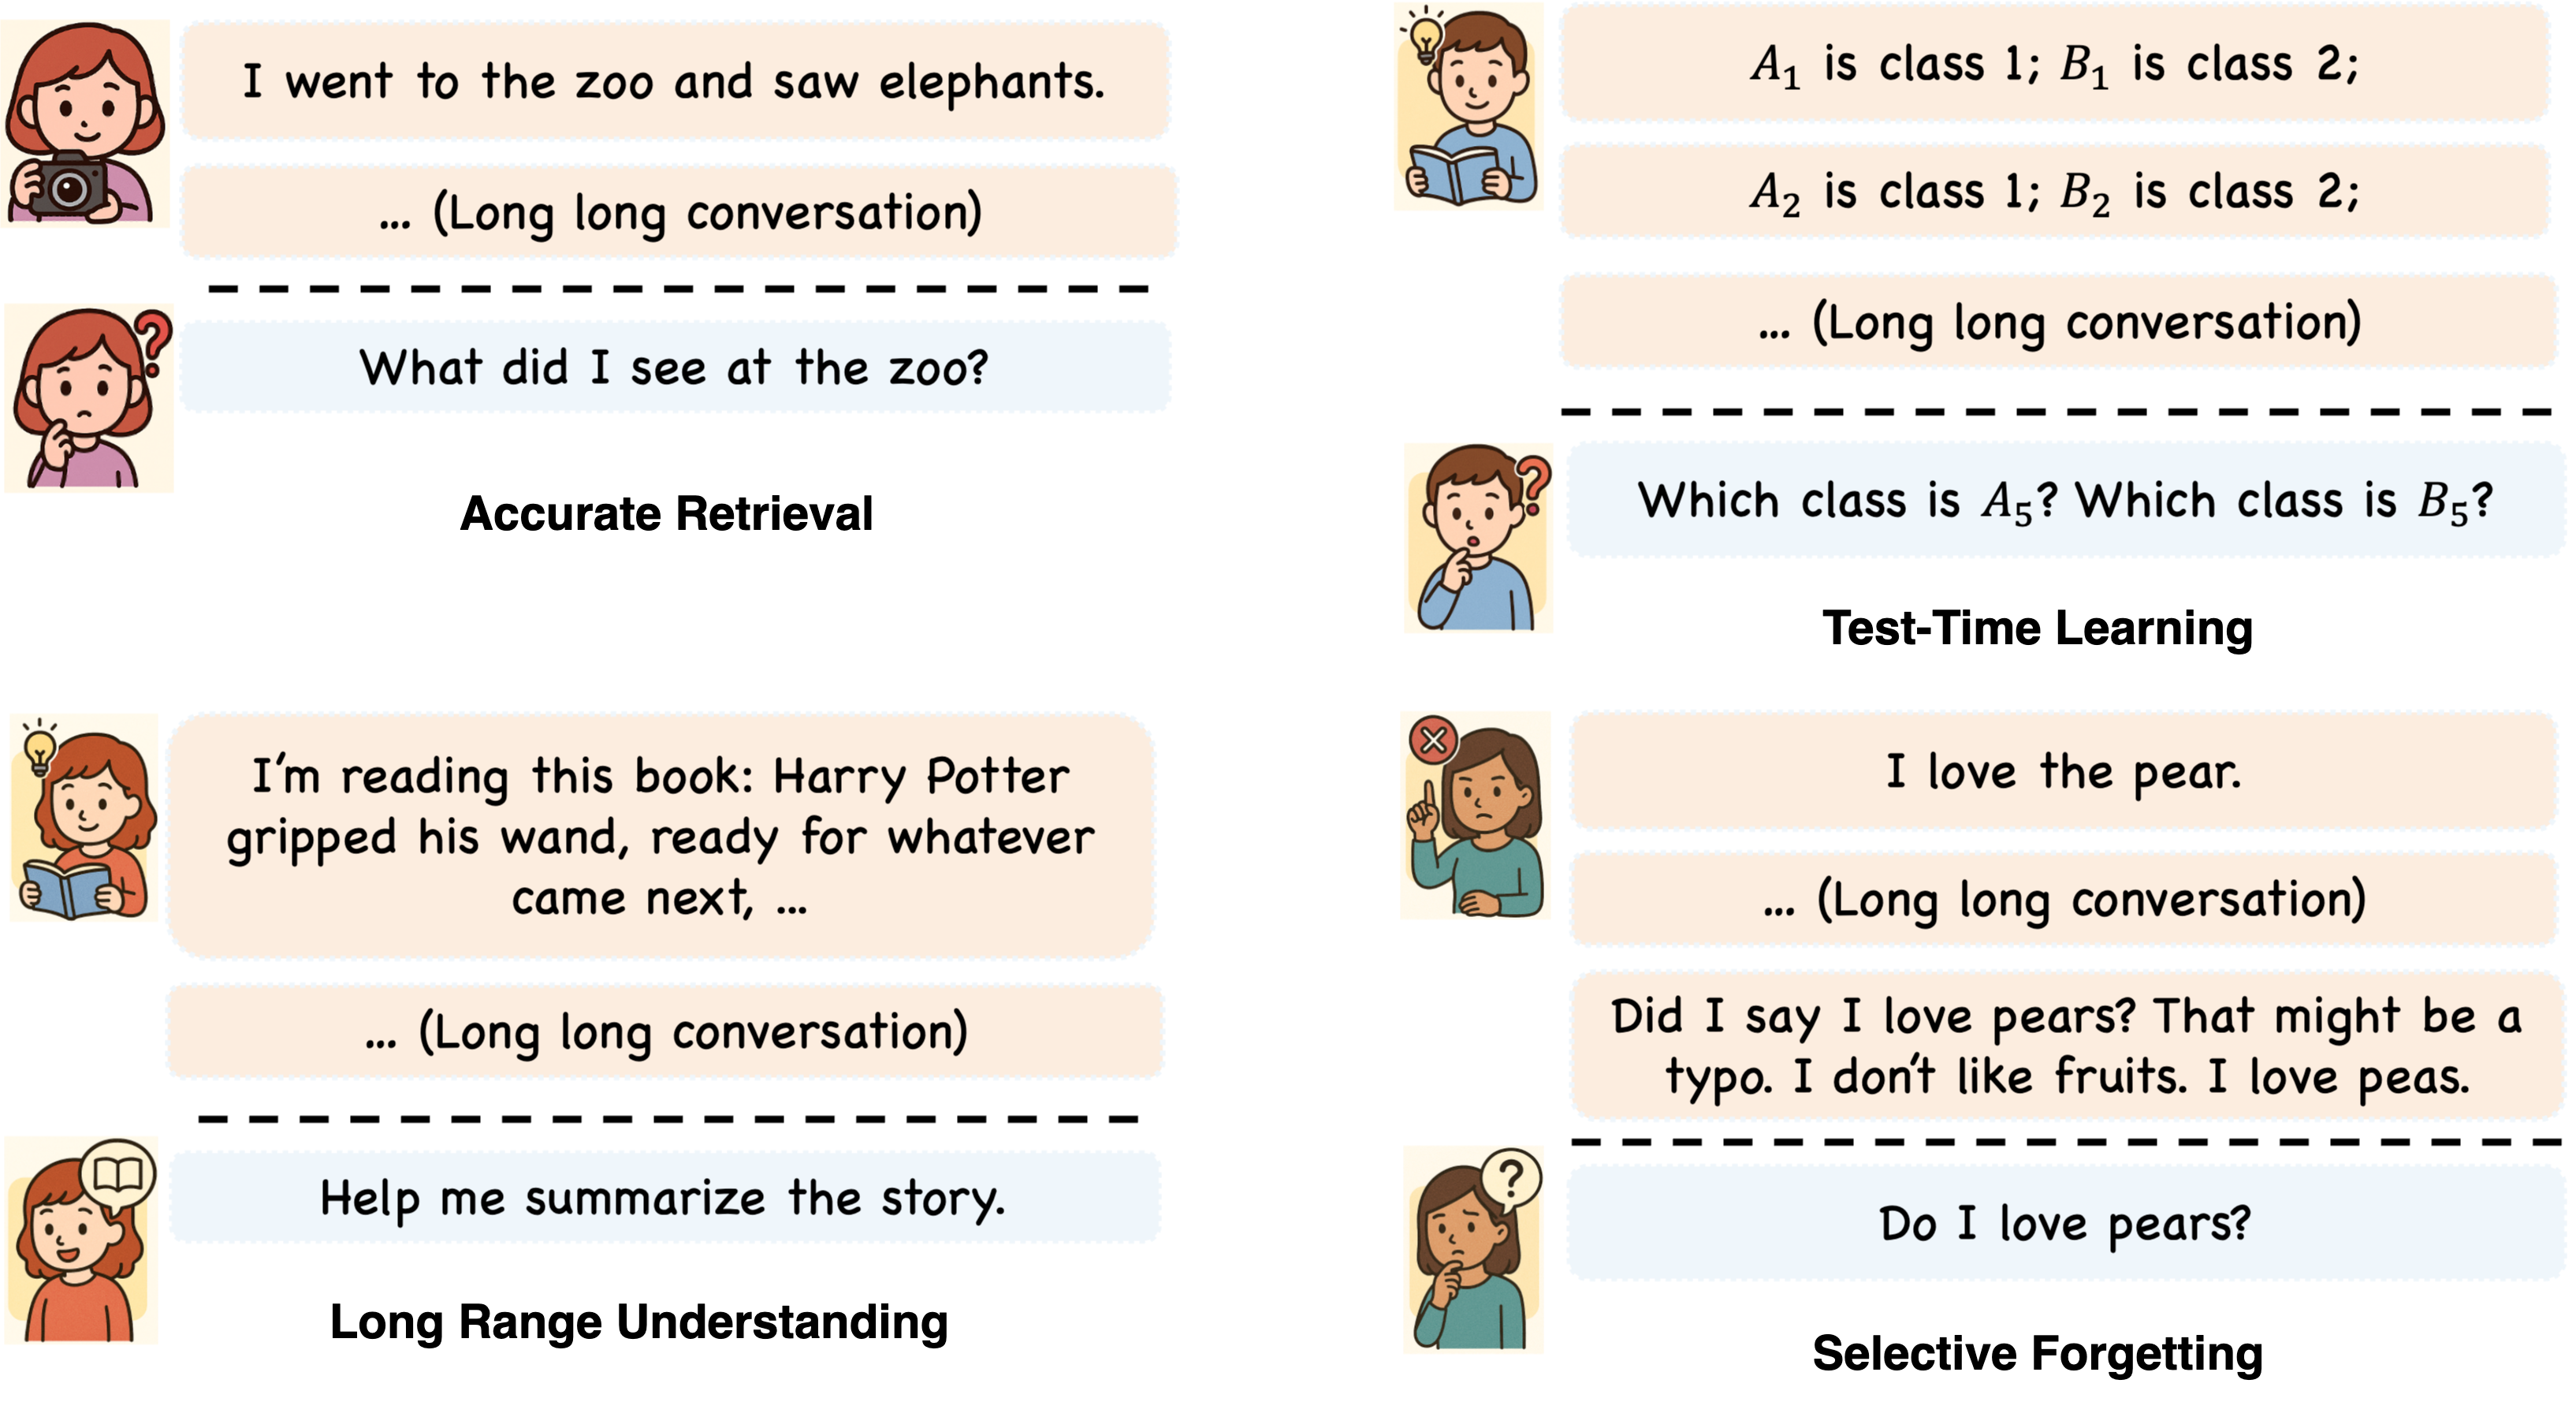
\includegraphics[width=0.9\linewidth]{figures/intro2.png}
    \caption{Four complementary competencies that memory agents should have.}
    \label{fig:intro}
    \vspace{-10pt}
\end{figure}
 
Previous datasets developed to evaluate memory in language models have notable limitations. Early benchmarks such as \textsc{LOCOMO}~\citep{locomo} ($\sim$9k tokens), LooGLE\citep{LooGLE} ($\sim$24k tokens), and LongBench\citep{longbench} ($\sim$ 20k tokens) feature relatively short contexts that no longer challenge current models. More recent datasets like NovelQA\citep{novelqa} ($\sim$200k tokens), NOCHA\citep{nocha} ($\sim$127k tokens), Loong\citep{loong} ($\sim$100k tokens), and $\infty$-Bench\citep{infinitebench} ($\sim$150k tokens) extend the context length to evaluate global reasoning and retrieval capabilities. However, these datasets were primarily designed for evaluating long-context language models rather than memory agents. 
The reason that long-context benchmarks cannot be directly used to evaluate memory agents is as follows. There is a fundamental distinction between memory and long context: memory serves as a compressed and distilled representation of past information. Rather than storing all historical content verbatim, memory selectively extracts salient details, removes irrelevant information, and often incorporates new inferences derived from prior experiences. Consequently, \textbf{memory agents are designed to process context incrementally}—absorbing input piece by piece, abstracting and consolidating information over time, generating new inferences, and learning novel rules from accumulated history. For this reason, datasets that provide the entire context in a single block are not directly applicable to evaluating memory agents. A more recent effort, \textsc{LongMemEval}~\citep{longmemeval}, seeks to address this limitation by using synthetic long-form conversations, which can be injected into memory gradually, session by session. Nonetheless, its evaluation framework remains constrained by limited topical diversity and less realistic interaction patterns, reducing its applicability to real-world memory agent scenarios. 


To address these limitations, we introduce a unified benchmark, \textbf{\ours}, specifically designed to evaluate a broad spectrum of memory mechanisms in agent systems. We also provide a framework for memory agent evaluation. In this framework, agents are presented with sequences of textual inputs that simulate multi-turn interactions with users. We reconstructed existing datasets originally developed for long-context LLM evaluation by segmenting and reconstructing inputs into multiple dialogue chunks and feeding them incrementally to the agent in a time order. However, since these datasets do not fully capture all four targeted memory competencies, we also introduce two new datasets: \textbf{EventQA} and \textbf{FactConsolidation}, designed to evaluate accurate retrieval and selective forgetting, respectively.
Our benchmark includes evaluations of state-of-the-art commercial memory agents (such as MIRIX and MemGPT), long-context agents that treat the full input as memory, and RAG agents that extend their memory through retrieval methods. We examine how techniques developed for long-context models and RAG transfer to the memory agent setting. By providing a consistent evaluation protocol across diverse agent architectures and datasets, \ours delivers comprehensive insights into agent performance across the four core memory competencies. In Table~\ref{tab:benchmark-comparison}, we compare the \ours with previous representative benchmarks across multiple dimensions.

% \yuanzhe{please polish your paper carefully....}

Our contributions are summarized as follows:
\begin{itemize}[leftmargin=*]
\item \textbf{Datasets:} We reconstruct existing datasets and create two new datasets to construct a comprehensive benchmark, covering four distinct memory competencies. 
\item \textbf{Framework:} We provide a unified evaluation framework, and open-source the codebase and datasets to encourage reproducibility and further research. 
\item \textbf{Empirical Study:} We implement various simple agents with diverse memory mechanisms, adopt commercial agents, and evaluate these agents on our proposed benchmark. Our results demonstrate that existing memory agents, although effective in some tasks, still face significant challenges in certain aspects.
\end{itemize}